\begin{center}
\footnotesize\noindent\fbox{
	\parbox{\textwidth}{
	Utilizzare la function ell'Esercizio 4.1 per approssimare la funzione di Runge sull'intervallo \([-6, 6]\), su una partizione uniforme di \(n+1\) ascisse per \(n = 2, 4, 6, \ldots, 40\). Stimare le corrispondenti costanti di Lebesgue.
	}
}\end{center}

\noindent Di seguito i grafici che mostrano i polinomi interpolanti di grado \textit{n} calcolati usando come punti di interpolazione le ascisse equispaziate nell'intervallo \([-6, 6]\) (evidenziati in rosso), sovraimposti al grafico della funzione di Runge \(f(x) = \frac{1}{1+x^2}\) (in blu). \\


\noindent\small\begin{tabular}{l*{5}{c}}
\hspace{3.5cm}\(n=2\) & \(n=4\) \\
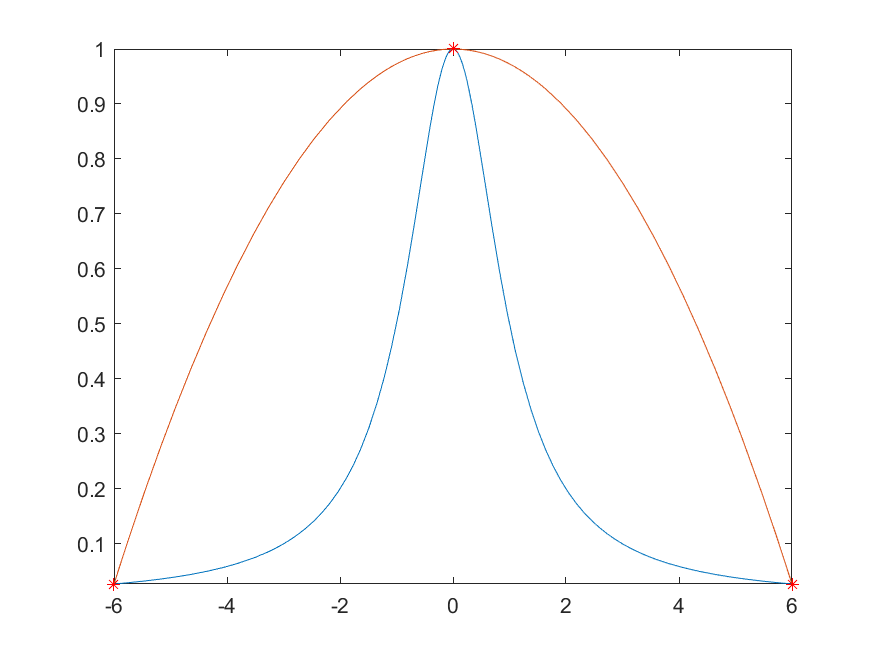
\includegraphics[scale=0.5]{cap4/4_9/2.png} &  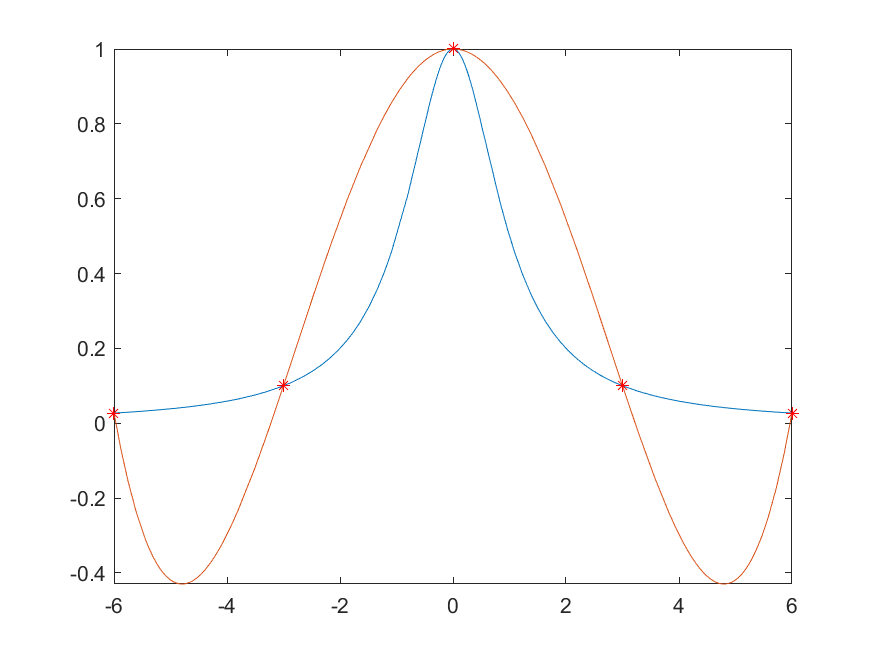
\includegraphics[scale=0.5]{cap4/4_9/4.png} \\

\hspace{3.5cm}\(n=6\)& \(n=8\) \\
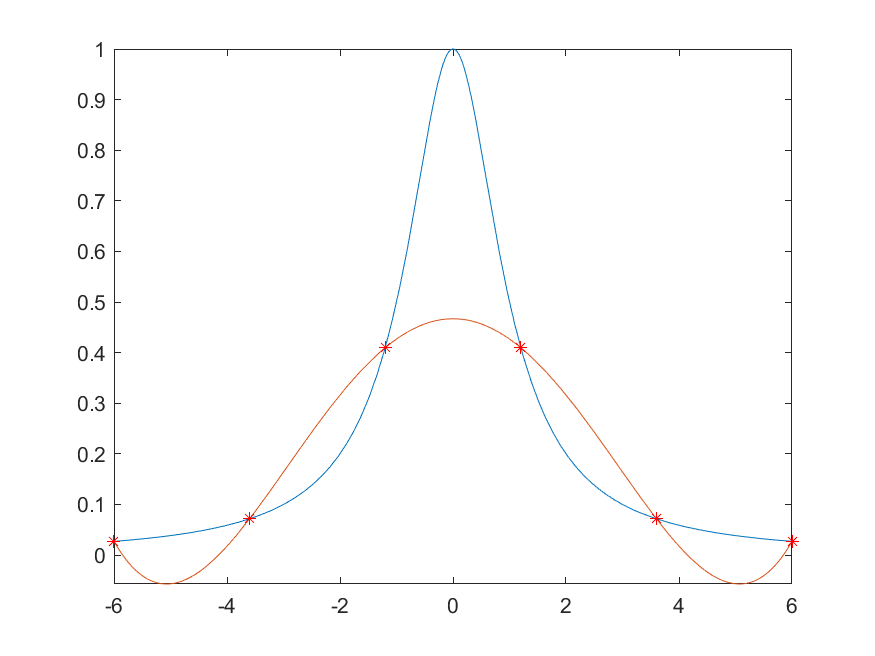
\includegraphics[scale=0.5]{cap4/4_9/6.png} &  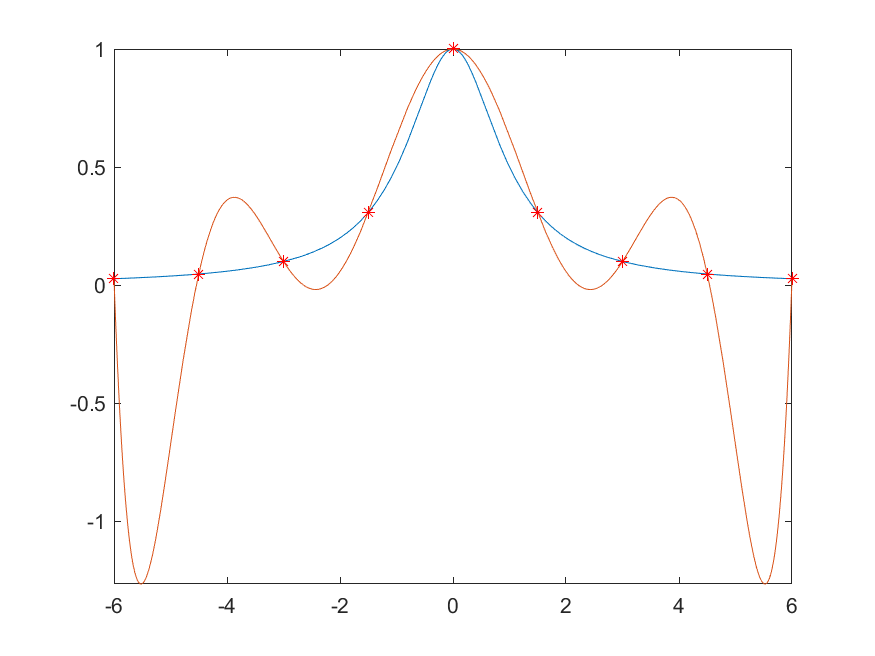
\includegraphics[scale=0.5]{cap4/4_9/8.png} \\

\hspace{3.5cm}\(n=10\) &  \(n=12\) \\
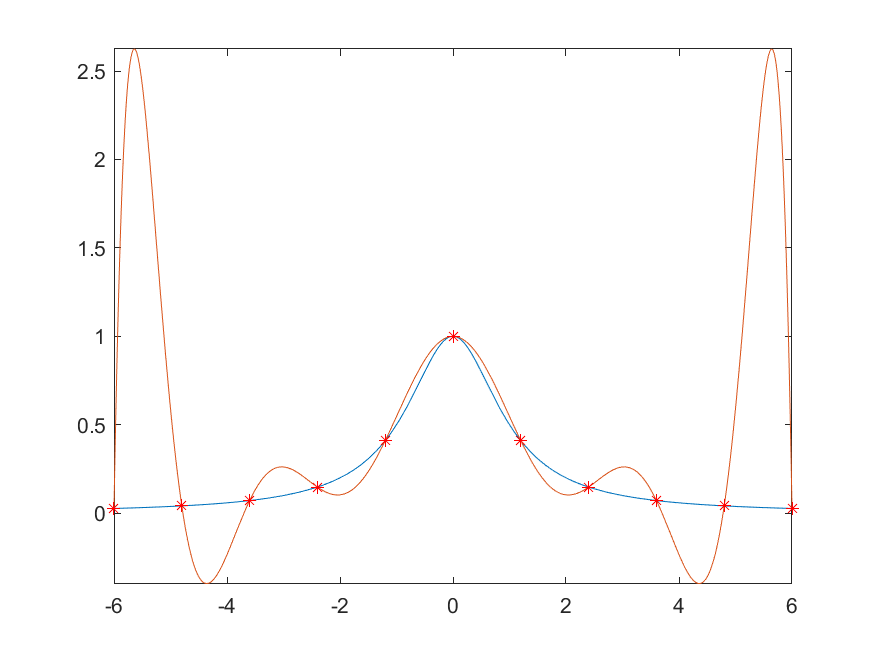
\includegraphics[scale=0.5]{cap4/4_9/10.png} &  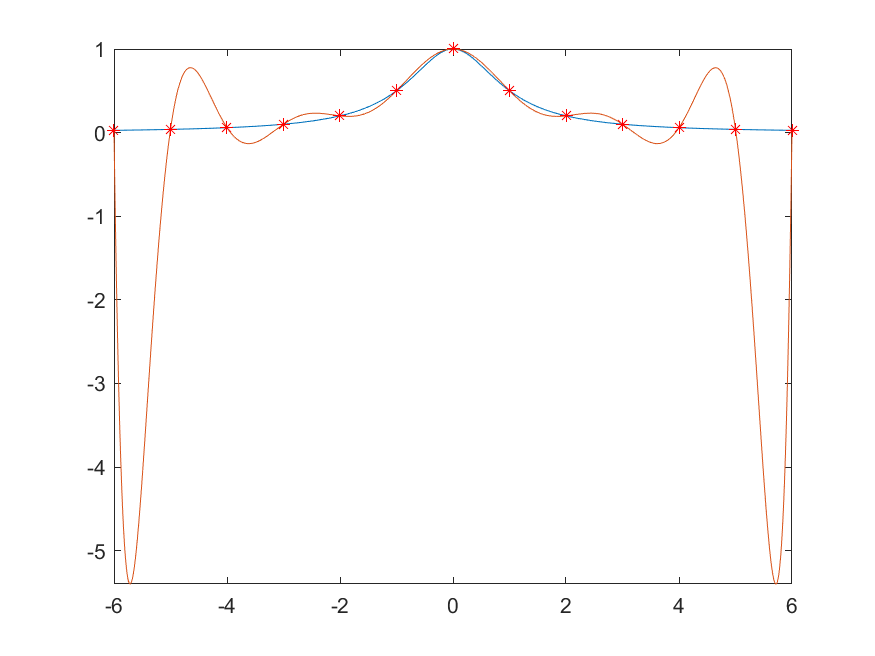
\includegraphics[scale=0.5]{cap4/4_9/12.png} \\
\end{tabular} \\ \\

\small\begin{tabular}{l*{5}{c}}
\hspace{3.5cm}\(n=14\) &  \(n=16\) \\
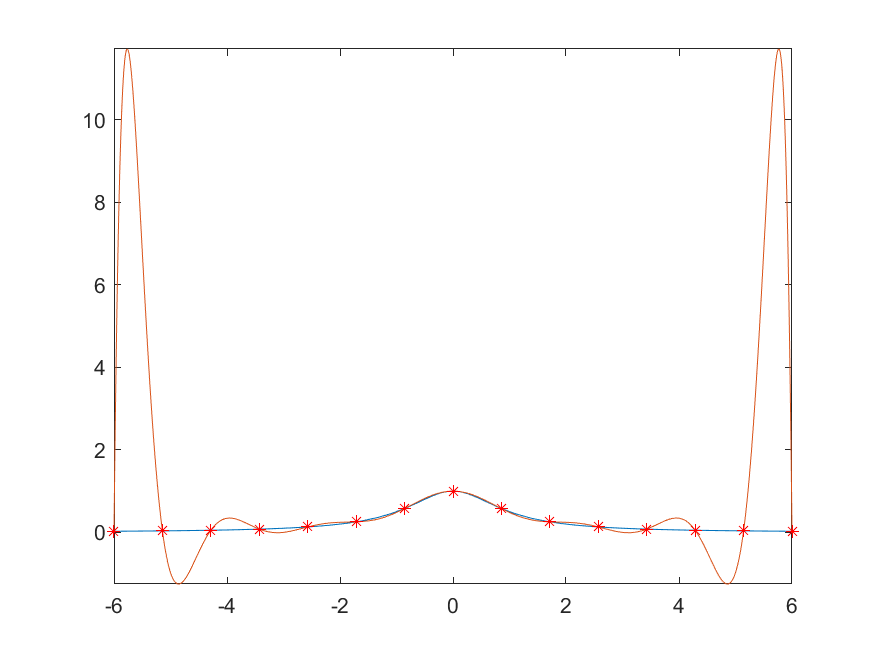
\includegraphics[scale=0.5]{cap4/4_9/14.png} &  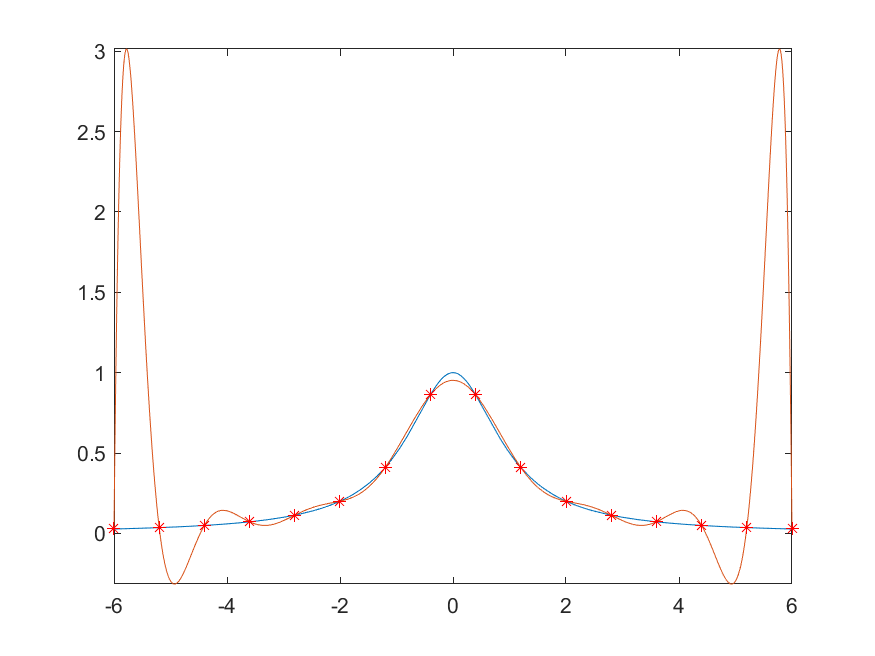
\includegraphics[scale=0.5]{cap4/4_9/16.png} \\

\hspace{3.5cm}\(n=18\) &  \(n=20\) \\
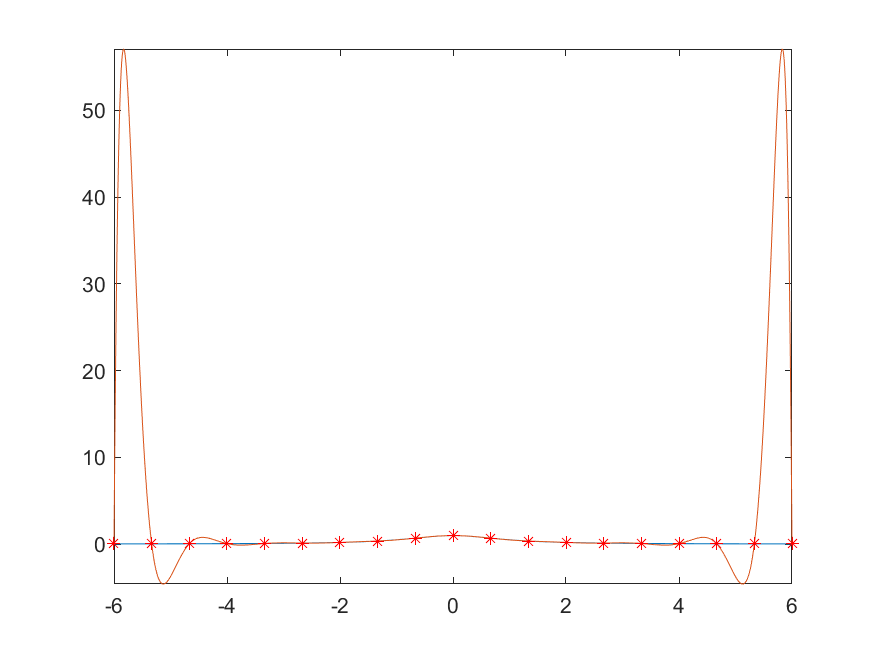
\includegraphics[scale=0.5]{cap4/4_9/18.png} &  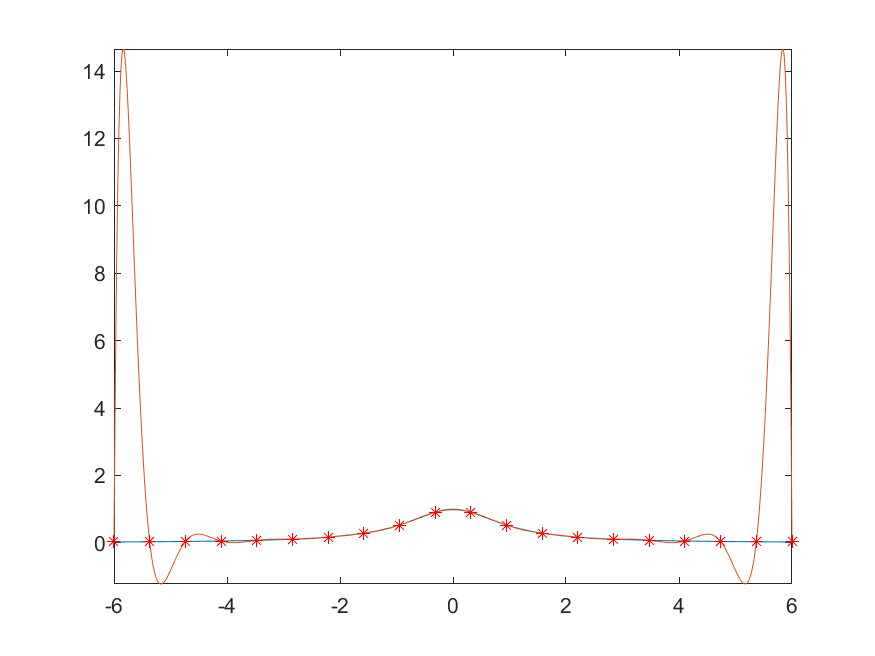
\includegraphics[scale=0.5]{cap4/4_9/20.png} \\

\hspace{3.5cm}\(n=22\) &  \(n=24\) \\
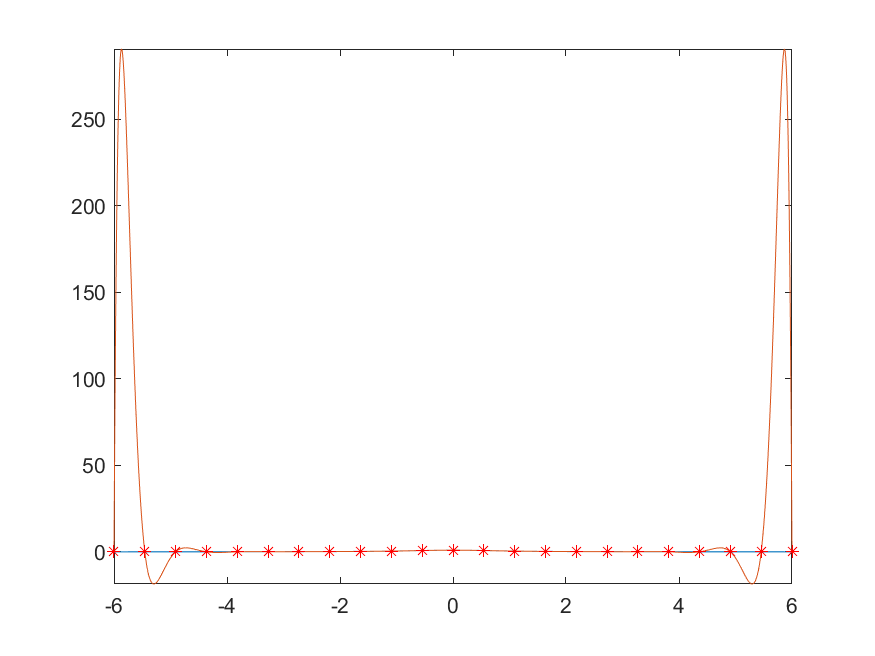
\includegraphics[scale=0.5]{cap4/4_9/22.png} &  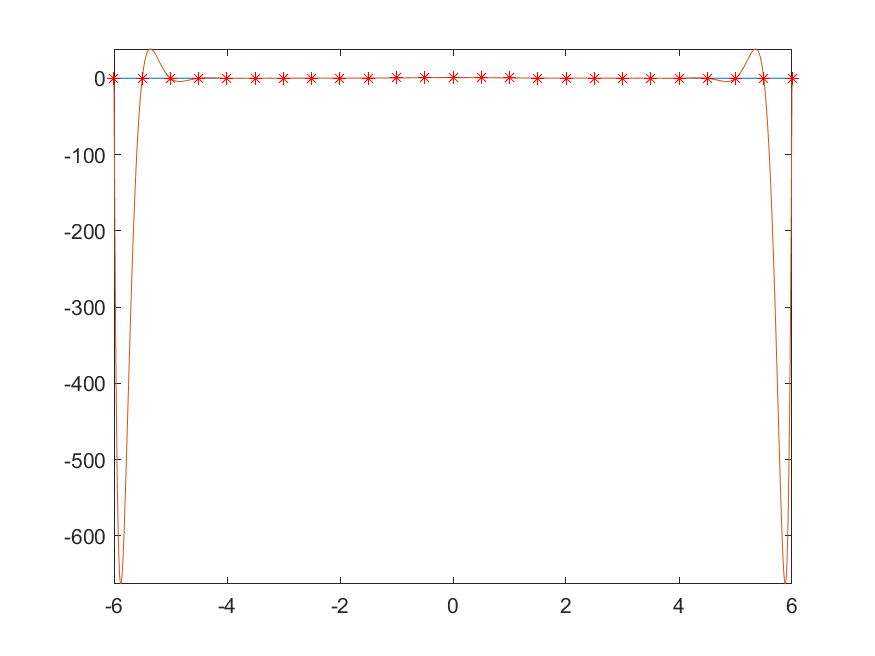
\includegraphics[scale=0.5]{cap4/4_9/24.png} \\

\hspace{3.5cm}\(n=26\) &  \(n=28\) \\
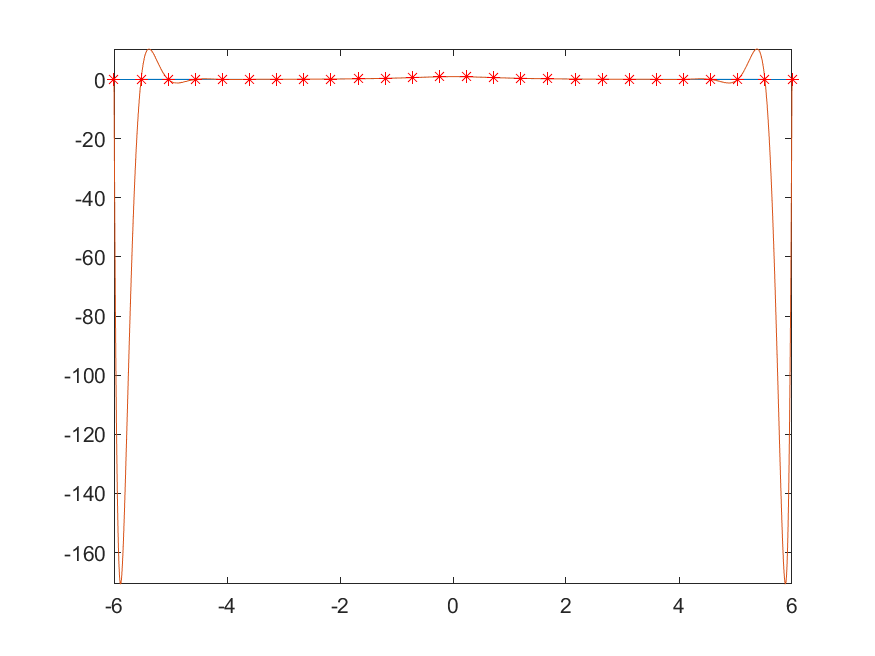
\includegraphics[scale=0.5]{cap4/4_9/26.png} &  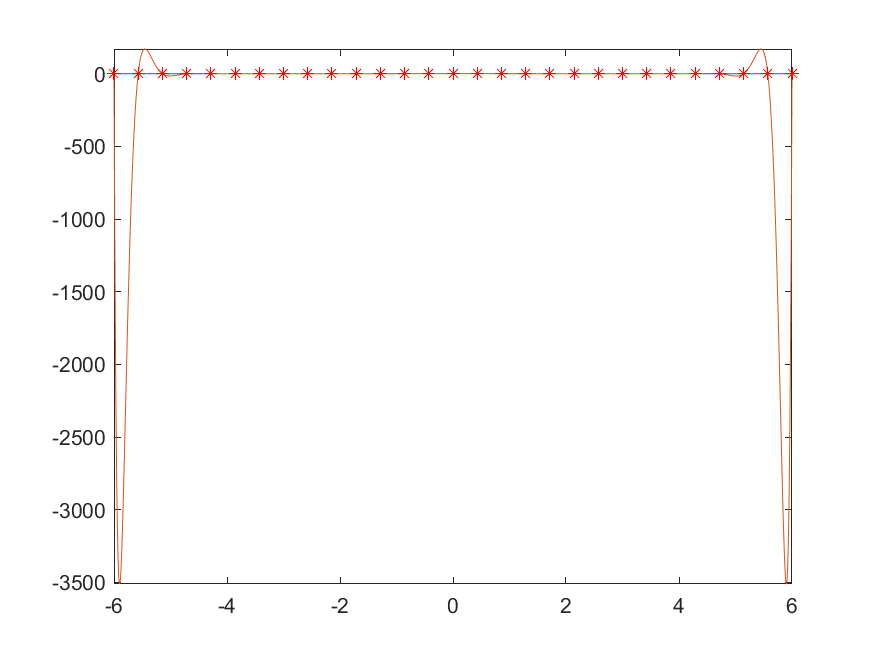
\includegraphics[scale=0.5]{cap4/4_9/28.png} \\
\end{tabular}

\small\begin{tabular}{l*{5}{c}}
\hspace{3.5cm}\(n=30\) &  \(n=32\) \\
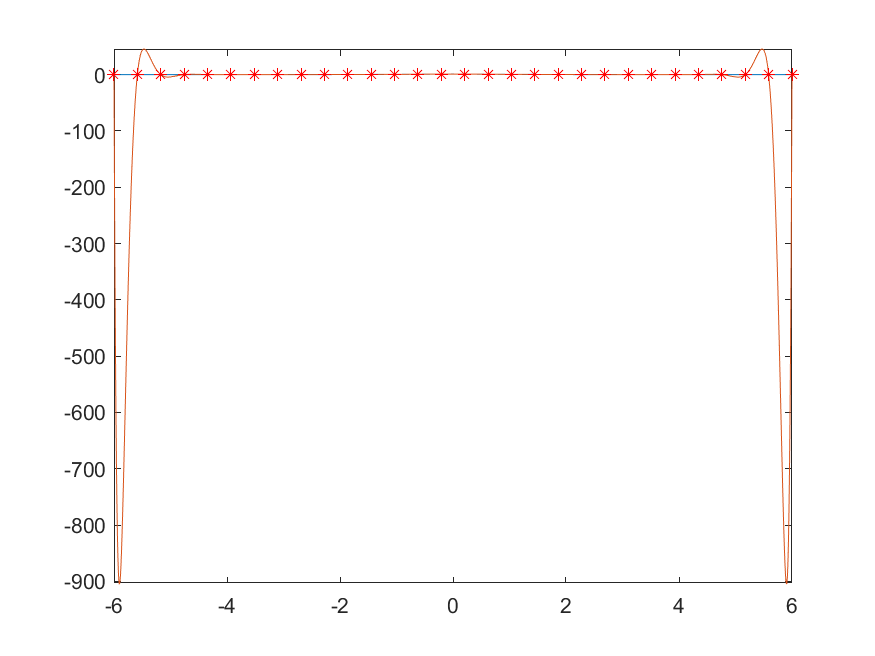
\includegraphics[scale=0.5]{cap4/4_9/30.png} &  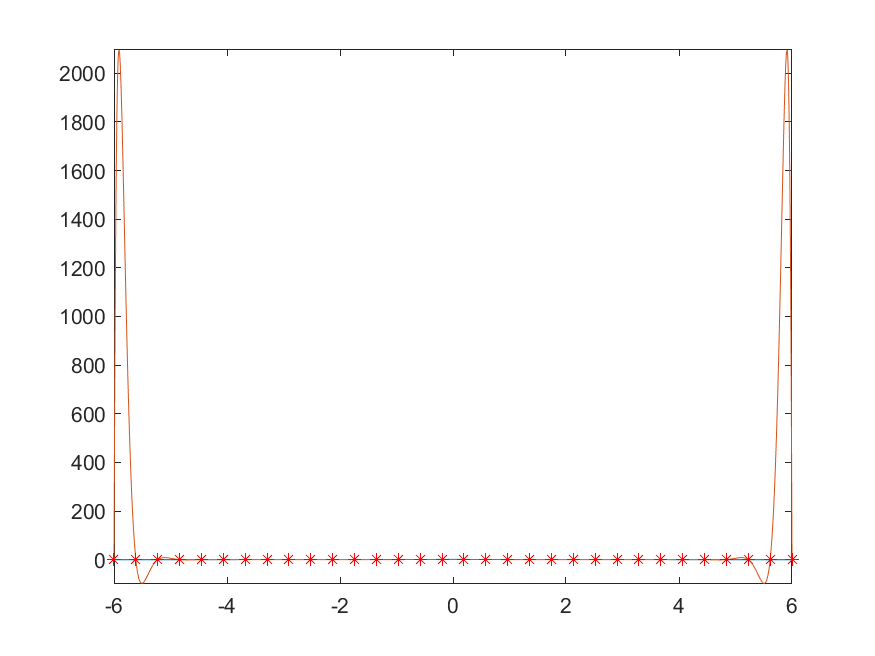
\includegraphics[scale=0.5]{cap4/4_9/32.png} \\

\hspace{3.5cm}\(n=34\) &  \(n=36\) \\
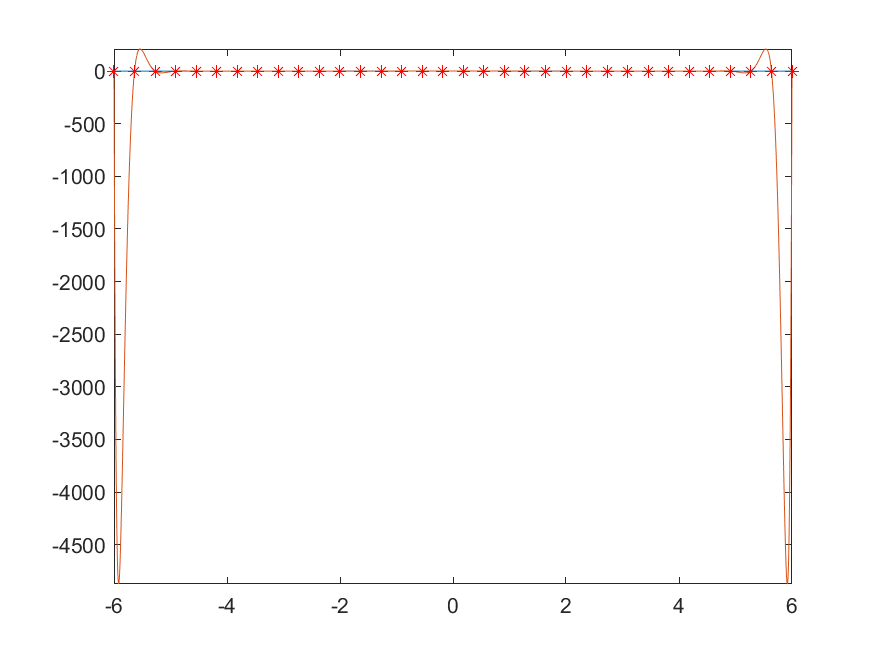
\includegraphics[scale=0.5]{cap4/4_9/34.png} &  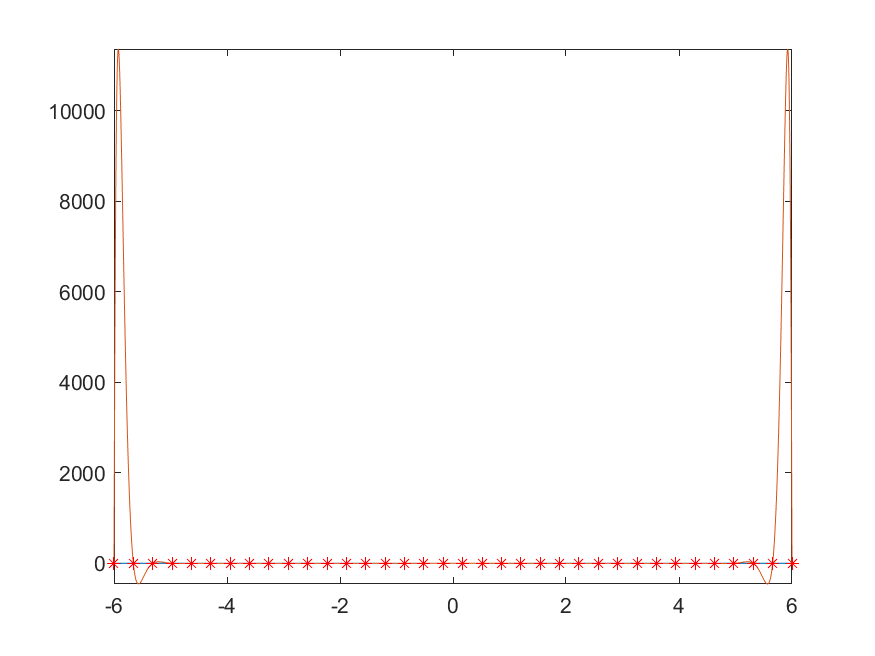
\includegraphics[scale=0.5]{cap4/4_9/36.png} \\

\hspace{3.5cm}\(n=38\) &  \(n=40\) \\
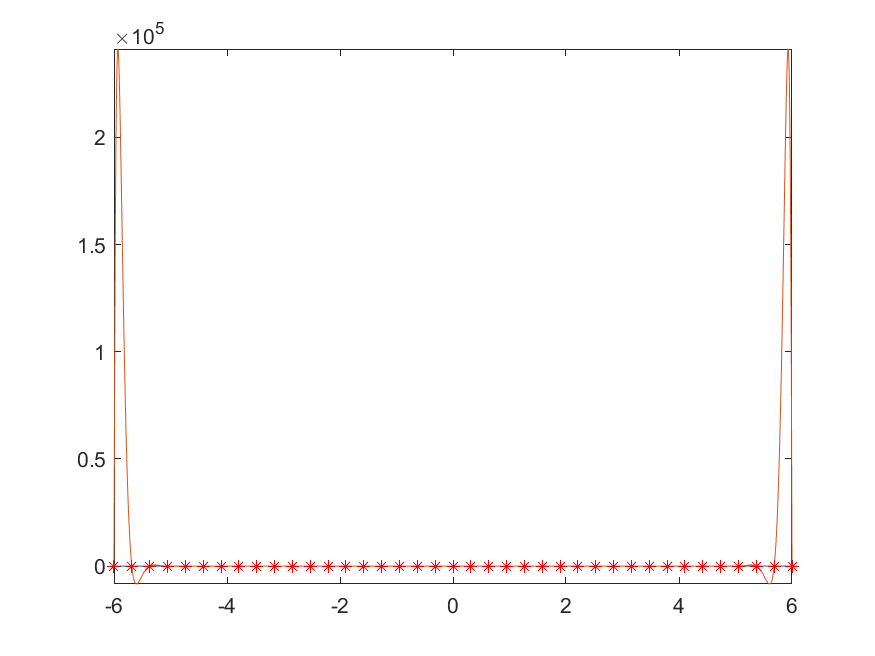
\includegraphics[scale=0.5]{cap4/4_9/38.png} &  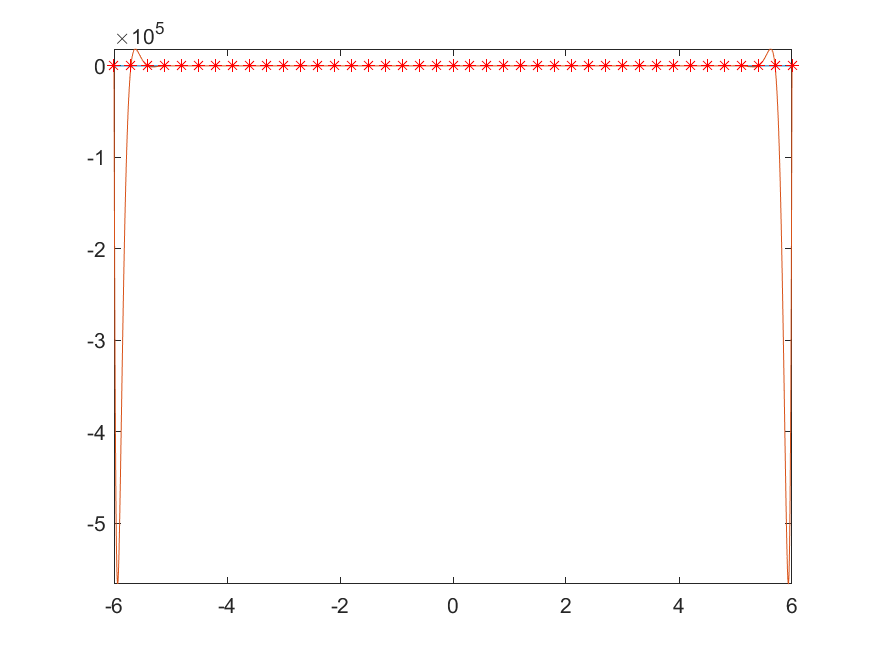
\includegraphics[scale=0.5]{cap4/4_9/40.png} \\
& \\
& \\
& \\
\end{tabular}

\noindent Riguardo alla stima della costante di Lebesgue in funzione di \(n\), ricordando che:

\[
\Delta_n \equiv ||\delta_n|| \equiv \sum^n_{k=0}|L_{k,n}(x)|
\]


\noindent Sono state calcolate le stime numeriche mostrate nella seguente tabella:

\begin{center}
	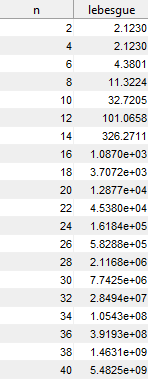
\includegraphics[scale=0.7]{cap4/4_9/4_9.png}
\end{center}

\noindent Il codice Matlab con cui sono stati realizzati i grafci e la tabella mostrati sopra \'e il seguente: \\

\lstinputlisting[language=Matlab]{cap4/4_9.m}
